  
  Uživatel má několik možností jak používat model \smod. Pomocí instalačního souboru lze nainstalovat \smod jako běžný Python balíček. Model \smod je rovněž poskytovaný jako zdrojový kód, kde se provádí instalaci běžným způsobem. Je rovněž možné spouštět balíček přímo bez instalace. V této částí manuálu je popsán první a nejjednodušší způsob, instalace pomocí instalačního souboru. 
  
  Model \smod je distribuován pod GPLv3\footnote{Více informací na: \href{https://www.gnu.org/licenses/gpl-3.0.en.html}{gnu.org/licenses/gpl-3.0.en.html}} licencí. Samotný kód modelu \smod je vydáván na stránkách  Katedra \pozn{katedra nebo Katedra} hydromeliorací a krajinného inženýrství Fakulty stavební ČVUT v Praze ...\pozn{odkaz}. Vývojové verze modelu jsou poskytovány na stránkách ...\pozn{odkaz, github - asi zalozit github instituce at to neni na uctu jerabekjak} stejně jako zdrojový kód tohoto manuálu. 
  
  Spustitelný instalační souboru pro operační systém Windows lze stáhnout na odkazu..\pozn{dopln}. Po spuštění toto souboru se spustí průvodce k instalaci standardního balíčku Python (úvodní obrazovka průvodce je ukázána na obrázku~\ref{fig:pruvodce}). Po ukončení instalace lze model \smod importovat do Python skriptu příkazem {\tt import smoderp2d.main}. 

  Před použitím modelu se doporučuje provést test, který ověří, zda má uživatel nainstalované ostatní balíčky, které model \smod používá. Testovací skript je spolu s testovacími daty ke stažení na adrese ...\pozn{adresa dopln} v adresáři {\tt tests}. Testovací skript s názvem {\tt importrun.py} uložte do společné složky s testovacími daty {\tt test-data}. Po spuštění skripty se otevře okno terminálu příkazové řádky. Pokud instalace malíčku \smod neproběhla nebo proběhla chybně, vypíše testovací skript hlášení ukázané na obrázku~\ref{fig:importerror}. Pokud nainstalované jiné nezbytné může se chybové hlášení lišit. Pokud například chybí balíček {\tt numpy} vypíše se na třetí řádek hlášení: {\tt No module named numpy}. V takovém případě je nutné chybějící balíčky doinstalovat běžným způsobem. Pokud proběhne testovací běh modelu \smod bezchybně, proběhne v okně terminálu hlášení ukázané na obrázku~\ref{fig:testok}. Výstupní soubory jsou pak uložený do složky {\tt test-out} v adresáři kde je uložen skript {\tt importrun.py}. V tento moment je model \smod i nezbytné malíčky zdárně nainstalovaný a jsou připraveny k použití.
  
  \begin{figure}[t!]
    \centering
    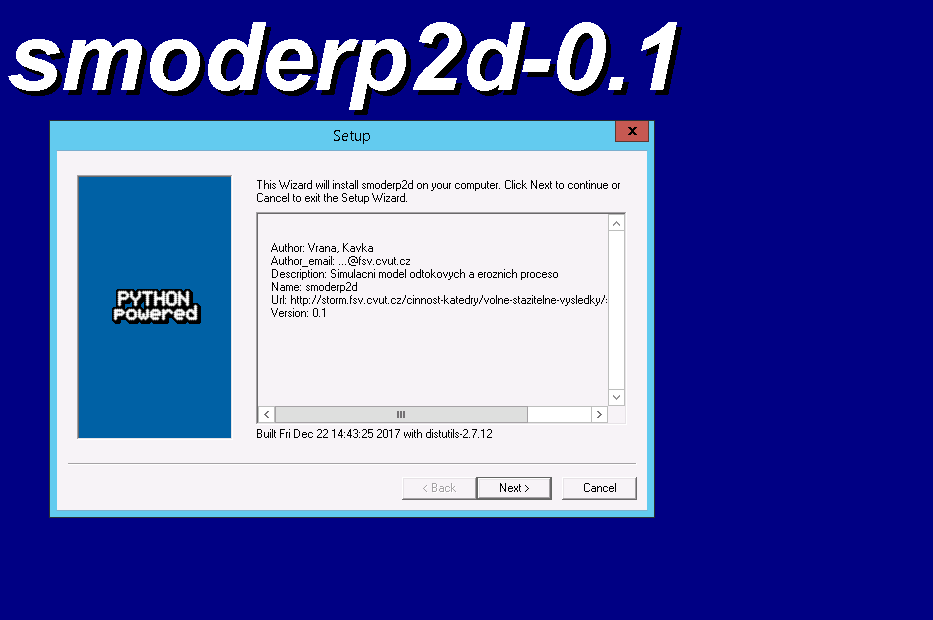
\includegraphics[width=0.75\textwidth]{./img/instalace.png}
    \caption{Úvodní obrazovka při instalaci malíčku \smod}
    \label{fig:pruvodce}
  \end{figure}
% 
  \begin{figure}[b!]
    \centering
    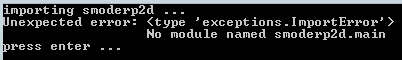
\includegraphics[width=0.75\textwidth]{./img/importerror.png}
    \caption{Hlášení při chybné instalaci malíčku modelu \smod}
    \label{fig:importerror}
  \end{figure}
% 
  \begin{figure}[t!]
    \centering
    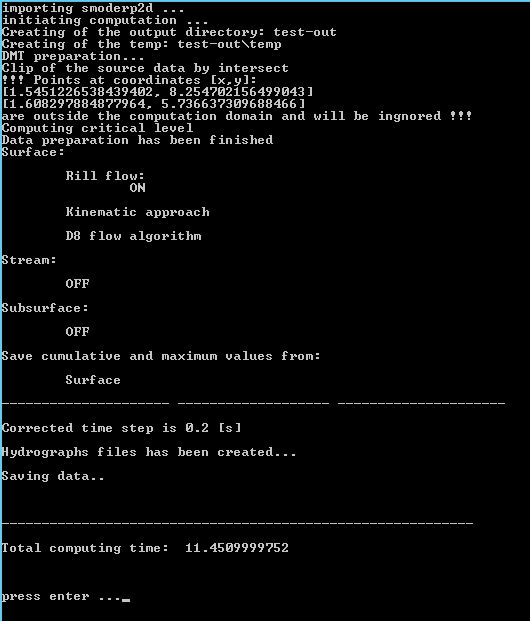
\includegraphics[width=0.75\textwidth]{./img/testok.png}
    \caption{Zdárný průběh testovacího skriptu modelu}
    \label{fig:testok}
  \end{figure}
  
\subsection{Použití modelu v ArcGIS}
  
  Současná verze modelu \smod využívá k přípravě vstupních dat výhradně software ArcGIS a Python malíček {\tt arcpy}. Proto je potřeba vytvořit spouštěcí skript, který načte a spustí model \smod. Takový skript může obsahovat následující příkazy:
%   \begin{figure}[h!]
    \begin{lstlisting}
      import smoderp2d.main as sm
      sm.run()
    \end{lstlisting}
%     \caption{Skript pro spuštění modelu \smod}
%   \end{figure}
  {\tt import smoderp2d.main as sm}  načte balíček modelu \smod. Spuštěním metody  {\tt sm.run()} je spuštěn samotný model. 
  
  Pro použití modelu v prostředí ArcGIS je třeba vytvořit ArcGIS {\tt toolbox}, kde je nastavený jako zdrojový soubor  uložený spouštěcí skript. Další krok je nastavení parametrů ArcGIS {\tt toolbox} odkud se načítají vstupní parametry do modelu. Pořadí zadávaných hodnot je {\bf nutné dodržet}! Ukázka ArcGIS {\tt toolbox} a vysvětlení parametrů je ukázáno na obrázku~\ref{fig:toolbox}. Připravený ArcGIS {\tt toolbox} lze sáhnout na stránce ...\pozn{odkaz}. Detailnější popis vstupních hodnot je v kapitole~\ref{kap:vstupy}.
  
  
  
  \begin{figure}[t!]
    \centering
    \begin{minipage}[t]{.45\textwidth}
      \centering
      \vspace{0pt}
      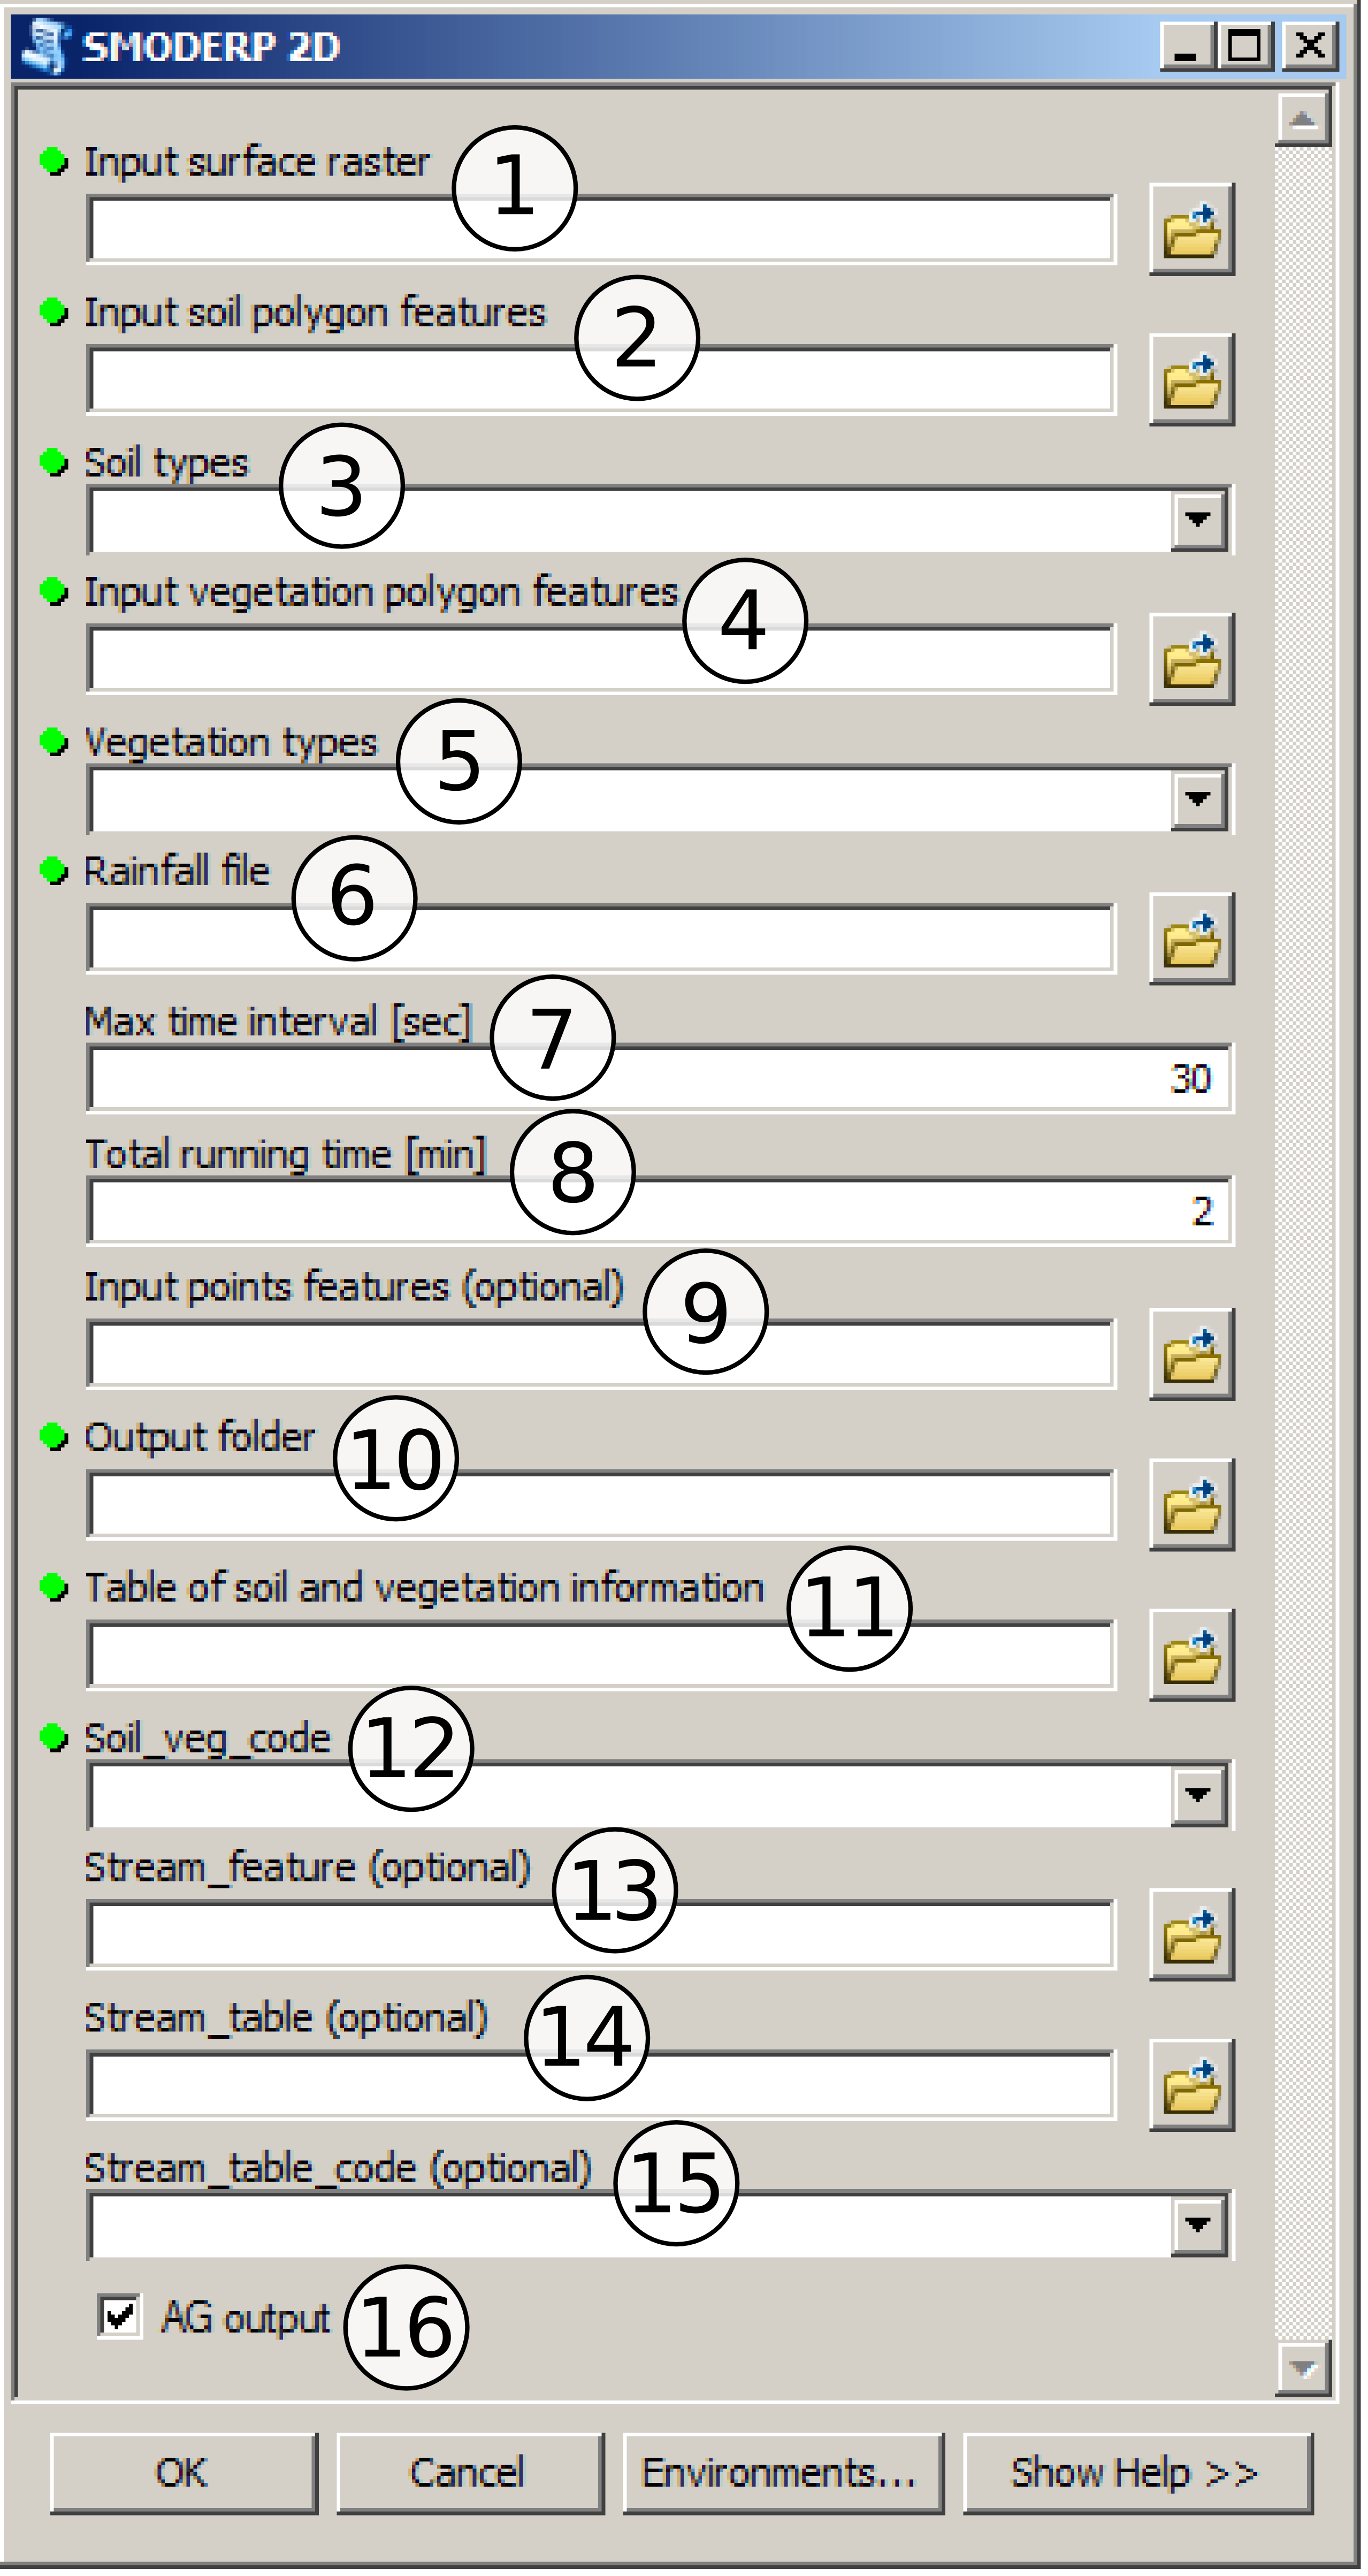
\includegraphics[width=\textwidth]{./img/toolboxpopis2.png}
    \end{minipage}\hfill
    \begin{minipage}[t]{.55\textwidth}
      \centering
      \vspace{0pt}
      {\scriptsize\sffamily
      \begin{tabular}{lp{.5\textwidth}l}
	\circled{1}  & Cesta k digitálnímu modlu terénu &  dopln typ primenne \\
	\circled{2}  & Cesta k vektorové vrstvě rozložení typu půd &  dopln typ primenne \\
	\circled{3}  & Název pole s id typů půd &  dopln typ primenne \\
	\circled{4}  & Cesta k vektorové vrstvě využití území &  dopln typ primenne \\
	\circled{5}  & Název pole s id využití území &  dopln typ primenne \\
	\circled{6}  & Cesta k souboru se srážkovými daty &  dopln typ primenne \\
	\circled{7}  & Maximální časový krok &  dopln typ primenne \\
	\circled{8}  & Konečný čas výpočtu &  dopln typ primenne \\
	\circled{9}  & Vrstva bodů pro výpis hydrogramů &  dopln typ primenne \\
	\circled{10} & Výstupní adresář &  dopln typ primenne \\
	\circled{11} & Tabulka s parametry modelu &  dopln typ primenne \\
	\circled{12} & Označení pole v tabulce \circled{11} &  dopln typ primenne \\
	\circled{13} & Cesta k vrstvě linií hydrografické sítě &  dopln typ primenne \\
	\circled{14} & Cesta k tabulce s geometrií úseků hydrografické sítě &  dopln typ primenne \\
	\circled{15} & Název společného pole pro spojení \circled{13} a \circled{14} &  dopln typ primenne \\
	\circled{16} & Volba formy výstupních souborů &  dopln typ primenne \\
      \end{tabular}
      }
    \end{minipage}
    \label{fig:toolbox}
    \caption{ArcGIS {\tt toolbox} a vysvětlenými parametry}
  \end{figure}
%     \centering
%     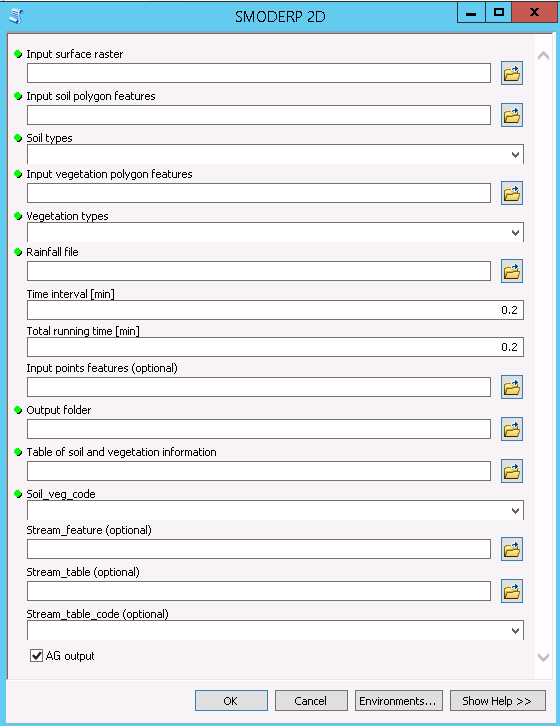
\includegraphics[width=0.75\textwidth]{./img/toolbox.png}
  
  
  
  
  